\ifx\pdfminorversion\undefined\else\pdfminorversion=4\fi
\documentclass[aspectratio=169,t,table]{beamer}
%\documentclass[aspectratio=169,t,handout]{beamer}

% English version FAU Logo
\usepackage[english]{babel}
% German version FAU Logo
%\usepackage[ngerman]{babel}

\usepackage[utf8]{inputenc}
\usepackage[T1]{fontenc}
\usepackage{amsmath,amssymb}
\usepackage{graphicx}
\usepackage{listings}
\usepackage{url}
\usepackage{xcolor}
\usepackage{enumitem}
\usepackage{hyperref}
\usepackage{fontawesome}
\usepackage{graphicx}
\usepackage{booktabs}
\usepackage{calc}
\usepackage{ifthen}
\usepackage{xcolor}
\usepackage{tikz}
\usepackage{tikz-cd}
\usepackage{verbatim}
\usepackage{pgfplots,pgfplotstable,pgf-pie}
\usepackage{filecontents}
\newcommand{\plots}{0.611201}
\newcommand{\plotm}{2.19882}
\pgfplotsset{height=4cm,width=8cm,compat=1.16}
\pgfmathdeclarefunction{gauss}{2}{%
  \pgfmathparse{1/(#2*sqrt(2*pi))*exp(-((x-#1)^2)/(2*#2^2))}%
}

\tikzset{
    vertex/.style = {
        circle,
        fill            = black,
        outer sep = 2pt,
        inner sep = 1pt,
    }
}

\tikzset{
    mynode/.style={
        draw,
        thick,
        anchor=south west,
        minimum width=2cm,
        minimum height=1.3cm,
        align=center,
        inner sep=0.2cm,
        outer sep=0,
        rectangle split,
        rectangle split parts=2,
        rectangle split draw splits=false},
    reverseclip/.style={
        insert path={(current page.north east) --
            (current page.south east) --
            (current page.south west) --
            (current page.north west) --
            (current page.north east)}
    }
}

\tikzset{basic/.style={
        draw,
        rectangle split,
        rectangle split parts=2,
        rectangle split part fill={blue!20,white},
        minimum width=2.5cm,
        text width=2cm,
        align=left,
        font=\itshape
    },
    Diamond/.style={ diamond,
                      draw,
                      shape aspect=2,
                      inner sep = 2pt,
                      text centered,
                      fill=blue!10!white,
                      font=\itshape
                    }}


\tikzset{level 1/.append style={sibling angle=50,level distance = 165mm}}
\tikzset{level 2/.append style={sibling angle=20,level distance = 45mm}}
\tikzset{every node/.append style={scale=1}}

\usetikzlibrary{arrows,decorations.pathmorphing,backgrounds,fit,positioning,shapes.symbols,chains,intersections,snakes,positioning,matrix,mindmap,shapes.multipart,shapes,calc,shapes.geometric}

% read in data file


\newcommand{\MaxNumberX}{3}
\newcommand{\MaxNumberY}{5}
\newcommand{\tikzmark}[1]{\tikz[remember picture] \node[coordinate] (#1) {#1};}

\pgfplotstableread{data/iris.dat}\iris
\pgfplotstablegetrowsof{\iris}
\pgfplotsset{compat=1.14}
\pgfmathsetmacro\NumRows{\pgfplotsretval-1}
\definecolor{airforceblue}{rgb}{0.36, 0.54, 0.66}

\usepgfplotslibrary{groupplots}
% Options:
%  - inst:      Institute
%                 med:      MedFak FAU theme
%                 nat:      NatFak FAU theme
%                 phil:     PhilFak FAU theme
%                 rw:       RWFak FAU theme
%                 rw-jura:  RWFak FB Jura FAU theme
%                 rw-wiso:  RWFak FB WISO FAU theme
%                 tf:       TechFak FAU theme
%  - image:     Cover image on title page
%  - plain:     Plain title page
%  - longtitle: Title page layout for long title
\usetheme[%
  image,%
  longtitle,%
  tf
]{fau}

% Enable semi-transparent animation preview
\setbeamercovered{transparent}


\lstset{%
  language=Python,
  tabsize=2,
  basicstyle=\tt,
  keywordstyle=\color{blue},
  commentstyle=\color{green!50!black},
  stringstyle=\color{red},
  numbers=left,
  numbersep=0.5em,
  xleftmargin=1em,
  numberstyle=\tt
}


% Title, authors, and date
\title[KDD]{Chapter VI: Classification}
\subtitle{Knowledge Discovery in Databases}
\author[L.~Melodia]{Luciano Melodia M.A.}
% English version
\institute[Department]{Evolutionary Data Management, Friedrich-Alexander University Erlangen-Nürnberg}
% German version
%\institute[Lehrstuhl]{Lehrstuhl, Friedrich-Alexander-Universit\"at Erlangen-N\"urnberg}
\date{Summer semester 2021}
% Set additional logo (overwrites FAU seal)
%\logo{\includegraphics[width=.15\textwidth]{themefau/art/xxx/xxx.pdf}}
\begin{document}
  % Title
  \maketitle

  {
    \setbeamertemplate{footline}{}
    \begin{frame}{Chapter VI: Classification}
        \begin{itemize}
            \item \textbf{Classification: basic concepts.}
            \item Decision-tree induction.
            \item Bayes classification methods.
            \item Rule-based classification.
            \item Model evaluation and selection.
            \item Techniques to improve classification accuracy: ensemble methods.
            \item Summary.
        \end{itemize}
    \end{frame}
  }

  {
    \setbeamertemplate{footline}{}
    \begin{frame}{Supervised vs. unsupervised learning}
        \begin{itemize}
            \item \textbf{\color{airforceblue}Supervised learning (classification).}
            \begin{itemize}
              \item Supervision:
              \begin{itemize}
                \item The \textbf{training data} (observations, measurements, etc.) are accompanied by \textbf{labels} indicating the \textbf{class} of the observations.
                \item New data is classified based on a \textbf{model} created from the training data.
              \end{itemize}
            \end{itemize}
            \item \textbf{\color{airforceblue}Unsupervised learning (clustering).}
            \begin{itemize}
              \item The class labels of training data are unknown.
              \begin{itemize}
                \item Or rather, there are no training data.
              \end{itemize}
            \end{itemize}
            \begin{itemize}
              \item Given a set of measurements, observations, etc., \\ the goal is to find classes or clusters in the data.
              \begin{itemize}
                \item See next chapter.
              \end{itemize}
            \end{itemize}
        \end{itemize}
    \end{frame}
  }

  {
    \setbeamertemplate{footline}{}
    \begin{frame}{Prediction problems: classification vs. numerical prediction}
        \begin{itemize}
            \item \textbf{Classification:}
            \begin{itemize}
              \item Predicts \textbf{\color{airforceblue}categorical class labels} (discrete, nominal).
              \item Constructs a model based on the training set and the values (class labels) in a classifying attribute and uses it in classifying new data.
            \end{itemize}
            \item \textbf{Numerical prediction:}
            \begin{itemize}
              \item Models \textbf{\color{airforceblue}continuous-valued functions}.
              \item I.e. predicts missing or unknown (future) values.
            \end{itemize}
            \item \textbf{Typical applications of classification:}
            \begin{itemize}
              \item Credit/loan approval: Will it be paid back?
              \item Medical diagnosis: Is a tumor cancerous or benign?
              \item Fraud detection: Is a transaction fraudulent or not?
              \item Web-page categorization: Which category is it?
            \end{itemize}
        \end{itemize}
    \end{frame}
  }

  {
    \setbeamertemplate{footline}{}
    \begin{frame}{Classification -- a two-step process}
        \begin{itemize}
            \item \textbf{Model construction: describing a set of predetermined classes:}
            \begin{itemize}
              \item Each tuple/sample is assumed to belong to a predefined class, as determined by the \textbf{\color{airforceblue}class-label attribute}.
              \item The set of tuples used for model construction is the \textbf{\color{airforceblue}training set}.
              \item The \textbf{\color{airforceblue}model} is represented as classification rules, decision trees, or mathematical formulae.
            \end{itemize}
            \item \textbf{Model usage, for classifying future or unknown objects:}
            \begin{itemize}
              \item Estimate \textbf{\color{airforceblue}accuracy} of the model:
              \begin{itemize}
                \item The known label of \textbf{test samples} is compared with the result from the model.
                \item \textbf{Accuracy rate} is the percentage of test-set samples that are correctly classified by the model.
                \item Test set is independent of training set (otherwise overfitting).
              \end{itemize}
              \item If the accuracy is acceptable, \textbf{\color{airforceblue}use the model} to classify data tuples whose class labels are not known.
            \end{itemize}
        \end{itemize}
    \end{frame}
  }

  {
    \setbeamertemplate{footline}{}
    \begin{frame}{Classification -- a two-step process}
      \centering
      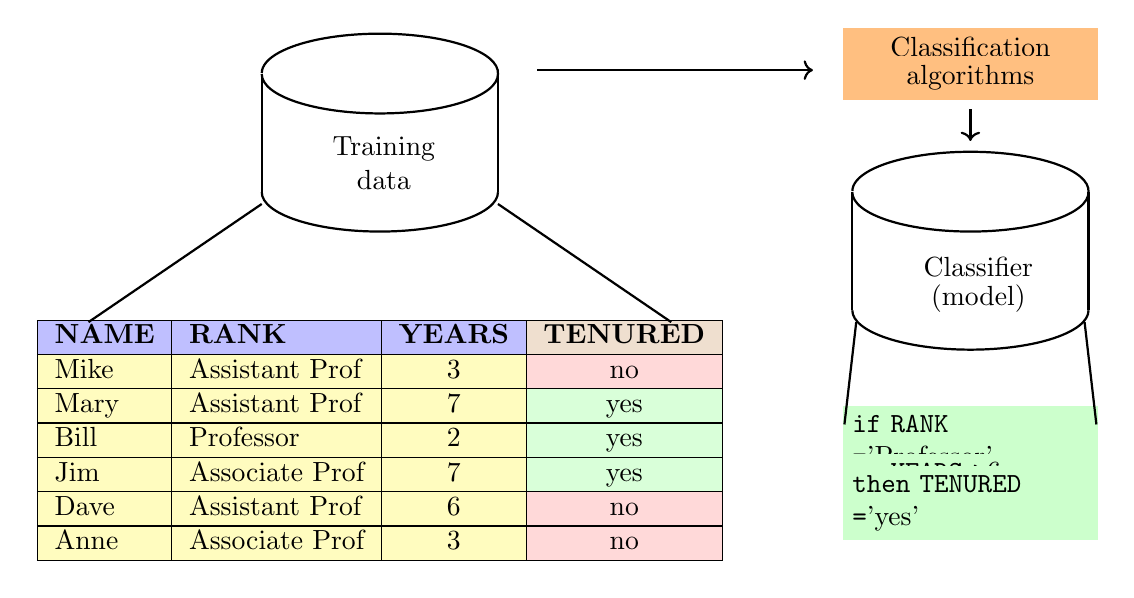
\begin{tikzpicture}
        \node at (0,0) {
        \begin{tabular}{|l|l|c|c|}
          \hline
          \cellcolor{blue!25}\textbf{\uppercase{name}} & \cellcolor{blue!25}\textbf{\uppercase{rank}} & \cellcolor{blue!25}\textbf{\uppercase{years}} & \cellcolor{brown!25}\textbf{\uppercase{tenured}} \\\hline
          \cellcolor{yellow!25}Mike & \cellcolor{yellow!25}Assistant Prof & \cellcolor{yellow!25}3 & \cellcolor{red!15}no \\\hline
          \cellcolor{yellow!25}Mary & \cellcolor{yellow!25}Assistant Prof & \cellcolor{yellow!25}7 & \cellcolor{green!15}yes \\\hline
          \cellcolor{yellow!25}Bill & \cellcolor{yellow!25}Professor & \cellcolor{yellow!25}2 & \cellcolor{green!15}yes \\\hline
          \cellcolor{yellow!25}Jim & \cellcolor{yellow!25}Associate Prof & \cellcolor{yellow!25}7 & \cellcolor{green!15}yes \\\hline
          \cellcolor{yellow!25}Dave & \cellcolor{yellow!25}Assistant Prof & \cellcolor{yellow!25}6 & \cellcolor{red!15}no \\\hline
          \cellcolor{yellow!25}Anne & \cellcolor{yellow!25}Associate Prof & \cellcolor{yellow!25}3 & \cellcolor{red!15}no \\\hline
        \end{tabular}
        };
        \node[fill=orange!50, text width = 3cm, align=center] at (7.5,5) {Classification};
        \node[fill=orange!50, text width = 3cm, align=center] at (7.5,4.6) {algorithms};

        \node[fill=green!20, text width = 3cm, align=left] at (7.5,0) {\texttt{if RANK =}'Professor'};
        \node[fill=green!20, text width = 3cm, align=left] at (7.5,-0.4) {\texttt{or YEARS >}6};
        \node[fill=green!20, text width = 3cm, align=left] at (7.5,-0.8) {\texttt{then TENURED =}'yes'};

        \node[text width = 3cm, align=center] at (0.05,3.7) {Training};
        \node[text width = 3cm, align=center] at (0.05,3.3) {data};

        \node[text width = 3cm, align=center] at (7.6,2.2) {Classifier};
        \node[text width = 3cm, align=center] at (7.6,1.8) {(model)};

        \draw [thick](-1.5,3.15) -- (-1.5,4.65);
        \draw [thick](1.5,3.15) -- (1.5,4.65);
        \draw [thick](-1.5,3.15) arc (180:360:1.5 and 0.5);
        \draw [thick](-1.5,4.65) arc (180:360:1.5 and 0.5);
        \draw [thick](1.5,4.65) arc (-1.5:180:1.5 and 0.5);
        \draw [thick, ->] (2,4.7) -- (5.5,4.7);
        \draw [thick, ->] (7.5,4.2) -- (7.5,3.8);
        \draw [thick] (6.05,1.5) -- (5.9,0.2);
        \draw [thick] (8.95,1.5) -- (9.1,0.2);

        \draw [thick](6,1.65) -- (6,3.15);
        \draw [thick](9,1.65) -- (9,3.15);
        \draw [thick](6,1.65) arc (180:360:1.5 and 0.5);
        \draw [thick](6,3.15) arc (180:360:1.5 and 0.5);
        \draw [thick](9,3.15) arc (-1.5:180:1.5 and 0.5);
        \draw [thick] (-3.7,1.5) -- (-1.5,3);
        \draw [thick] (1.5,3) -- (3.7,1.5);
      \end{tikzpicture}
    \end{frame}
  }

  {
    \setbeamertemplate{footline}{}
    \begin{frame}{Process (II): using the model in prediction}
      \centering
      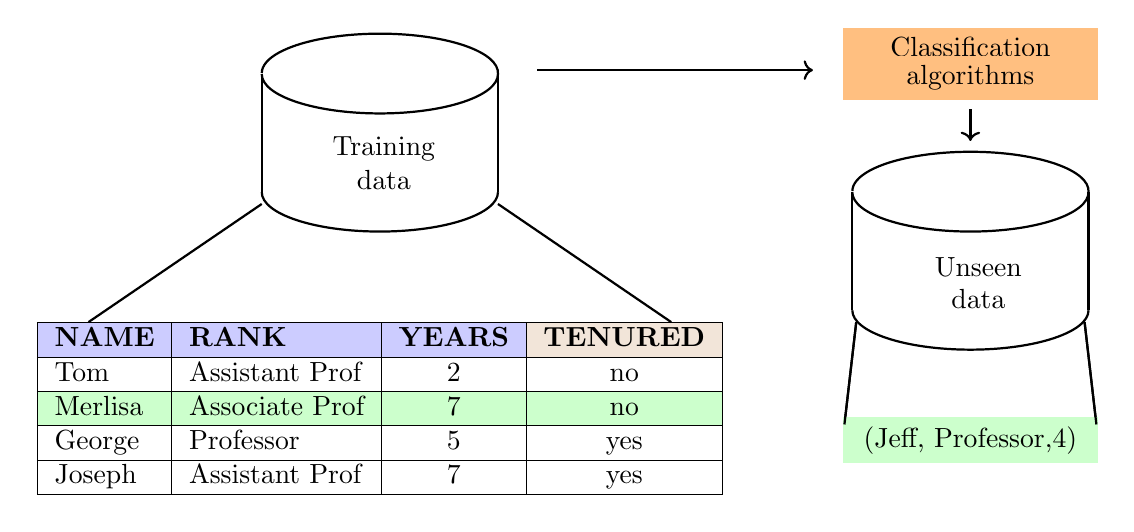
\begin{tikzpicture}
        \draw [thick](-1.5,3.15) -- (-1.5,4.65);
        \draw [thick](1.5,3.15) -- (1.5,4.65);
        \draw [thick](-1.5,3.15) arc (180:360:1.5 and 0.5);
        \draw [thick](-1.5,4.65) arc (180:360:1.5 and 0.5);
        \draw [thick](1.5,4.65) arc (-1.5:180:1.5 and 0.5);
        \draw [thick, ->] (2,4.7) -- (5.5,4.7);
        \draw [thick, ->] (7.5,4.2) -- (7.5,3.8);
        \draw [thick] (6.05,1.5) -- (5.9,0.2);
        \draw [thick] (8.95,1.5) -- (9.1,0.2);
        \node[text width = 3cm, align=center] at (0.05,3.7) {Training};
        \node[text width = 3cm, align=center] at (0.05,3.3) {data};

        \node[text width = 3cm, align=center] at (7.6,2.2) {Unseen};
        \node[text width = 3cm, align=center] at (7.6,1.8) {data};

        \node at (0,0.4){
        \begin{tabular}{|l|l|c|c|}
          \hline
          \cellcolor{blue!20}\textbf{\uppercase{name}} & \cellcolor{blue!20}\textbf{\uppercase{rank}} & \cellcolor{blue!20}\textbf{\uppercase{years}} & \cellcolor{brown!20}\textbf{\uppercase{tenured}} \\\hline
          Tom & Assistant Prof & 2 & no \\\hline
          \cellcolor{green!20}Merlisa & \cellcolor{green!20}Associate Prof & \cellcolor{green!20}7 & \cellcolor{green!20}no \\\hline
          George & Professor & 5 & yes \\\hline
          Joseph & Assistant Prof & 7 & yes \\\hline
        \end{tabular}
        };
        \node[fill=orange!50, text width = 3cm, align=center] at (7.5,5) {Classification};
        \node[fill=orange!50, text width = 3cm, align=center] at (7.5,4.6) {algorithms};
        \node[fill=green!20, text width = 3cm, align=center] at (7.5,0) {(Jeff, Professor,4)};
        \draw [thick] (6.05,1.5) -- (5.9,0.2);
        \draw [thick] (8.95,1.5) -- (9.1,0.2);
        \draw [thick](6,1.65) -- (6,3.15);
        \draw [thick](9,1.65) -- (9,3.15);
        \draw [thick](6,1.65) arc (180:360:1.5 and 0.5);
        \draw [thick](6,3.15) arc (180:360:1.5 and 0.5);
        \draw [thick](9,3.15) arc (-1.5:180:1.5 and 0.5);
        \draw [thick] (-3.7,1.5) -- (-1.5,3);
        \draw [thick] (1.5,3) -- (3.7,1.5);
      \end{tikzpicture}
    \end{frame}
  }

  {
    \setbeamertemplate{footline}{}
    \begin{frame}{Chapter VI: Classification}
        \begin{itemize}
            \item Classification: basic concepts.
            \item \textbf{Decision-tree induction.}
            \item Bayes classification methods.
            \item Rule-based classification.
            \item Model evaluation and selection.
            \item Techniques to improve classification accuracy: ensemble methods.
            \item Summary.
        \end{itemize}
    \end{frame}
  }

  {
    \setbeamertemplate{footline}{}
    \begin{frame}{Decision-tree induction: an example}
      \begin{columns}
        \begin{column}{0.4\textwidth}
          \vspace{-3cm}
          \begin{itemize}
            \item \textbf{Training dataset: buys\_computer.}
            \begin{itemize}
              \item The dataset follows an example of Quinlan's ID3 (playing tennis).
            \end{itemize}
            \item \textbf{Resulting tree:}\\[0.1cm]
            \centering
            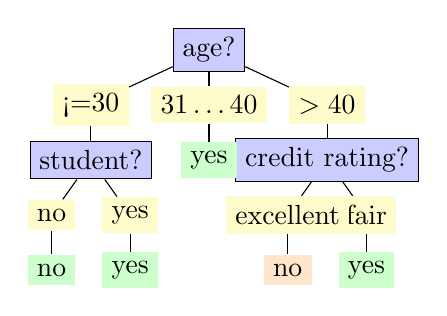
\begin{tikzpicture}
              \node[draw, fill=blue!20] at (0,0) (a) {age?};
              \node[fill=yellow!20] at (-1.5,-0.7) (b) {<=30};
              \node[fill=yellow!20] at (0,-0.7) (c) {$31\ldots40$};
              \node[fill=yellow!20] at (1.5,-0.7) (d) {$>40$};
              \node[draw, fill=blue!20] at (-1.5,-1.4) (e) {student?};
              \node[fill=yellow!20] at (-2,-2.1) (eno1) {no};
              \node[fill=yellow!20] at (-1,-2.1) (eyes1) {yes};
              \node[fill=green!20] at (-2,-2.8) (eno2) {no};
              \node[fill=green!20] at (-1,-2.8) (eyes2) {yes};
              \node[draw, fill=blue!20] at (1.5,-1.4) (g) {credit rating?};
              \node[fill=yellow!20] at (2,-2.1) (gf) {fair};
              \node[fill=yellow!20] at (1,-2.1) (gex) {excellent};
              \node[fill=orange!20] at (1,-2.8) (gno) {no};
              \node[fill=green!20] at (2,-2.8) (gyes) {yes};
              \node[fill=green!20] at (0,-1.4) (f) {yes};

              \draw (a)--(b);
              \draw (a)--(c);
              \draw (a)--(d);
              \draw (b)--(e);
              \draw (c)--(f);
              \draw (d)--(g);
              \draw (e)--(eno1);
              \draw (e)--(eyes1);
              \draw (eno1)--(eno2);
              \draw (eyes1)--(eyes2);
              \draw (g)--(gex);
              \draw (g)--(gf);
              \draw (gex)--(gno);
              \draw (gf)--(gyes);
            \end{tikzpicture}
          \end{itemize}
        \end{column}
        \begin{column}{0.6\textwidth}
          \begin{tabular}{|l|l|c|c|c|}
            \hline
            \cellcolor{blue!20}age & \cellcolor{blue!20}income & \cellcolor{blue!20}student & \cellcolor{blue!20}credit\_rating & \cellcolor{blue!20}buys\_coputer \\\hline
            \cellcolor{yellow!20}$\leq 30$ & \cellcolor{yellow!20}high & \cellcolor{yellow!20}no & \cellcolor{yellow!20}fair & \cellcolor{red!20}no \\\hline
            \cellcolor{yellow!20}$\leq 30$ & \cellcolor{yellow!20}high & \cellcolor{yellow!20}no & \cellcolor{yellow!20}excellent & \cellcolor{red!20}no \\\hline
            \cellcolor{yellow!20}$31\ldots40$ & \cellcolor{yellow!20}high & \cellcolor{yellow!20}no & \cellcolor{yellow!20}fair & \cellcolor{green!20}yes \\\hline
            \cellcolor{yellow!20}$>40$ & \cellcolor{yellow!20}medium & \cellcolor{yellow!20}no & \cellcolor{yellow!20}fair & \cellcolor{green!20}yes \\\hline
            \cellcolor{yellow!20}$>40$ & \cellcolor{yellow!20}low & \cellcolor{yellow!20}yes & \cellcolor{yellow!20}fair & \cellcolor{green!20}yes \\\hline
            \cellcolor{yellow!20}$>40$ & \cellcolor{yellow!20}low & \cellcolor{yellow!20}yes & \cellcolor{yellow!20}excellent & \cellcolor{red!20}no \\\hline
            \cellcolor{yellow!20}$31\ldots40$ & \cellcolor{yellow!20}low & \cellcolor{yellow!20}yes & \cellcolor{yellow!20}excellent & \cellcolor{green!20}yes \\\hline
            \cellcolor{yellow!20}$\leq 30$ & \cellcolor{yellow!20}medium & \cellcolor{yellow!20}no & \cellcolor{yellow!20}fair & \cellcolor{red!20}no \\\hline
            \cellcolor{yellow!20}$\leq 30$ & \cellcolor{yellow!20}low & \cellcolor{yellow!20}no & \cellcolor{yellow!20}fair & \cellcolor{green!20}yes \\\hline
            \cellcolor{yellow!20}$>40$ & \cellcolor{yellow!20}medium & \cellcolor{yellow!20}yes & \cellcolor{yellow!20}fair & \cellcolor{green!20}yes \\\hline
            \cellcolor{yellow!20}$\leq 30$ & \cellcolor{yellow!20}medium & \cellcolor{yellow!20}yes & \cellcolor{yellow!20}excellent & \cellcolor{green!20}yes \\\hline
            \cellcolor{yellow!20}$31\ldots40$ & \cellcolor{yellow!20}medium & \cellcolor{yellow!20}no & \cellcolor{yellow!20}excellent & \cellcolor{green!20}yes \\\hline
            \cellcolor{yellow!20}$31\ldots40$ & \cellcolor{yellow!20}high & \cellcolor{yellow!20}yes & \cellcolor{yellow!20}fair & \cellcolor{green!20}yes \\\hline
            \cellcolor{yellow!20}$>40$ & \cellcolor{yellow!20}medium & \cellcolor{yellow!20}no & \cellcolor{yellow!20}excellent & \cellcolor{red!20}no \\\hline
          \end{tabular}
        \end{column}
      \end{columns}
    \end{frame}
  }

  {
    \setbeamertemplate{footline}{}
    \begin{frame}{Algorithm for decision-tree induction}
        \begin{itemize}
            \item \textbf{Basic algorithm (a greedy algorithm):}
            \begin{itemize}
              \item Tree is constructed in a \textbf{\color{airforceblue}top-down recursive divide-and-conquer manner.}
              \item Attributes are categorical.
              \begin{itemize}
                \item If not: discretize in advance.
              \end{itemize}
              \item At start, all the training examples are at the root.
              \item Examples are \textbf{\color{airforceblue}partitioned recursively} based on selected attributes.
              \item Test attributes are selected on the basis of a heuristic or statistical measure.
              \begin{itemize}
                \item E.g. information gain -- see on the next slide.
              \end{itemize}
            \end{itemize}
            \item \textbf{Conditions for stopping partitioning:}
            \begin{itemize}
              \item All samples for a given node belong to the same class.
              \item There are no remaining attributes for further partitioning.
              \begin{itemize}
                \item Majority voting is employed for classifying the leaf.
              \end{itemize}
              \item There are no samples left (i.e. partition for particular value is empty).
            \end{itemize}
        \end{itemize}
    \end{frame}
  }

  {
    \setbeamertemplate{footline}{}
    \begin{frame}{Attribute-selection measure: information gain (ID3/C4.5)}
      \begin{itemize}
        \item \textbf{Select the attribute with the highest information gain.}
        \begin{itemize}
          \item Let $p_i$ be the probability that an arbitrary tuple in $D$ belings to class $C_i$,\\ estimated by $\frac{|C_i|}{|D|}$, such that $1 \leq i \leq m$.
          \item \textbf{Expected information} (entropy)needed to classify a tuple in $D$:
          \begin{align}
            \text{Info}(D) = -\sum_{i=1}^{m}p_i \log_2(p_i).
          \end{align}
          \item \textbf{Information} needed (after using attribute $A$ to split $D$ into $v$ partitions) to classify $D$:
          \begin{align}
            \text{Info}_A(D) = \sum_{j=1}^v \left( \frac{|D_j|}{|D|} \text{Info}(D_j) \right).
          \end{align}
          \item \textbf{Information gained} by branching on $A$:
          \begin{align}
            \text{Gain}(A)=\text{Info}(D)-\text{Info}_A(D).
          \end{align}
        \end{itemize}
      \end{itemize}
    \end{frame}
  }

  {
    \setbeamertemplate{footline}{}
    \begin{frame}{Attribute selection: information gain}
      \begin{columns}
        \begin{column}{0.45\textwidth}
          \begin{itemize}
            \item \textbf{Class P: buys\_computer = "yes"}
            \item \textbf{Class N: buys\_computer = "no"}
            \begin{align*}
              \resizebox{7cm}{!}{%
                $\text{Info}(D) = I(9,5) = - \frac{9}{14}\log_2(\frac{9}{14})-\frac{5}{14} \log_2(\frac{5}{14}) = 0.94$
              }
            \end{align*}
          \end{itemize}
          \centering
          \begin{tabular}{|l|l|l|l|}
            \hline
            \cellcolor{blue!20}age & \cellcolor{blue!20}p & \cellcolor{blue!20}n & \cellcolor{blue!20}$l(p,n)$ \\\hline
            \cellcolor{yellow!20}$\leq 30$ & 2 & 3 & 0.971 \\\hline
            \cellcolor{yellow!20}$31\ldots40$ & 4 & 0 & 0 \\\hline
            \cellcolor{yellow!20}$>40$ & 3 & 2 & 0.971 \\\hline
          \end{tabular}\\[0.2cm]
        \begin{itemize}
          \item \textbf{Similarly,}
          \begin{itemize}
            \item $\text{Gain}(\texttt{income}) = 0.029$,
            \item $\text{Gain}(\texttt{student}) = 0.151$,
            \item $\text{Gain}(\texttt{credit\_rating}) = 0.048$.
          \end{itemize}
        \end{itemize}
        \end{column}
        \begin{column}{0.45\textwidth}
          \vspace{-1.3cm}
          \begin{align*}
            \resizebox{7cm}{!}{%
              $\text{Info}_{\texttt{age}}(D) = \frac{5}{14}I(2,3) + \frac{4}{14} I(4,0) + \frac{5}{14} I(3,2) = 0.694$.
            }
          \end{align*}
          $\frac{5}{14} I(2,3)$ means "$\texttt{age} \leq 30$" has $5$ out of $14$ samples, with $2$ yes'es and $3$ no's. Hence,
          \begin{align*}
              \text{Gain}(\texttt{age}) = \text{Info}(D)-\text{Info}_{\texttt{age}}(D) = 0.246.
          \end{align*}
          \resizebox{\columnwidth}{!}{%
          \begin{tabular}{|l|l|c|l|c|}
            \hline
            \cellcolor{blue!20}age & \cellcolor{blue!20}income & \cellcolor{blue!20}student & \cellcolor{blue!20}credit\_rating & \cellcolor{brown!20}buys\_computer \\\hline
            \cellcolor{yellow!20}$\leq30$ & \cellcolor{yellow!20}high & \cellcolor{yellow!20}no & \cellcolor{yellow!20}fair & \cellcolor{red!20}no \\\hline
            \cellcolor{yellow!20}$\leq30$ & \cellcolor{yellow!20}high & \cellcolor{yellow!20}no & \cellcolor{yellow!20}excellent & \cellcolor{red!20}no \\\hline
            \cellcolor{yellow!20}$31\ldots40$ & \cellcolor{yellow!20}high & \cellcolor{yellow!20}no & \cellcolor{yellow!20}fair & \cellcolor{green!20}yes \\\hline
            \cellcolor{yellow!20}$>40$ & \cellcolor{yellow!20}medium & \cellcolor{yellow!20}no & \cellcolor{yellow!20}fair & \cellcolor{green!20}yes \\\hline
            \cellcolor{yellow!20}$>40$ & \cellcolor{yellow!20}low & \cellcolor{yellow!20}yes & \cellcolor{yellow!20}fair & \cellcolor{green!20}yes \\\hline
            \cellcolor{yellow!20}$>40$ & \cellcolor{yellow!20}low & \cellcolor{yellow!20}yes & \cellcolor{yellow!20}excellent & \cellcolor{red!20}no \\\hline
            \cellcolor{yellow!20}$31\ldots40$ & \cellcolor{yellow!20}low & \cellcolor{yellow!20}yes & \cellcolor{yellow!20}excellent & \cellcolor{green!20}yes \\\hline
            \cellcolor{yellow!20}$\leq30$ & \cellcolor{yellow!20}medium & \cellcolor{yellow!20}no & \cellcolor{yellow!20}fair & \cellcolor{red!20}no \\\hline
            \cellcolor{yellow!20}$>40$ & \cellcolor{yellow!20}medium & \cellcolor{yellow!20}yes & \cellcolor{yellow!20}fair & \cellcolor{green!20}yes \\\hline
            \cellcolor{yellow!20}$\leq30$ & \cellcolor{yellow!20}medium & \cellcolor{yellow!20}yes & \cellcolor{yellow!20}excellent & \cellcolor{green!20}yes \\\hline
            \cellcolor{yellow!20}$31\ldots40$ & \cellcolor{yellow!20}medium & \cellcolor{yellow!20}no & \cellcolor{yellow!20}fair & \cellcolor{green!20}yes \\\hline
            \cellcolor{yellow!20}$31\ldots40$ & \cellcolor{yellow!20}high & \cellcolor{yellow!20}yes & \cellcolor{yellow!20}fair & \cellcolor{green!20}yes \\\hline
            \cellcolor{yellow!20}$>40$ & \cellcolor{yellow!20}medium & \cellcolor{yellow!20}no & \cellcolor{yellow!20}excellent & \cellcolor{red!20}no \\\hline
          \end{tabular}}
        \end{column}
      \end{columns}
    \end{frame}
  }

  {
    \setbeamertemplate{footline}{}
    \begin{frame}{Partitioning in the example}
      \centering
      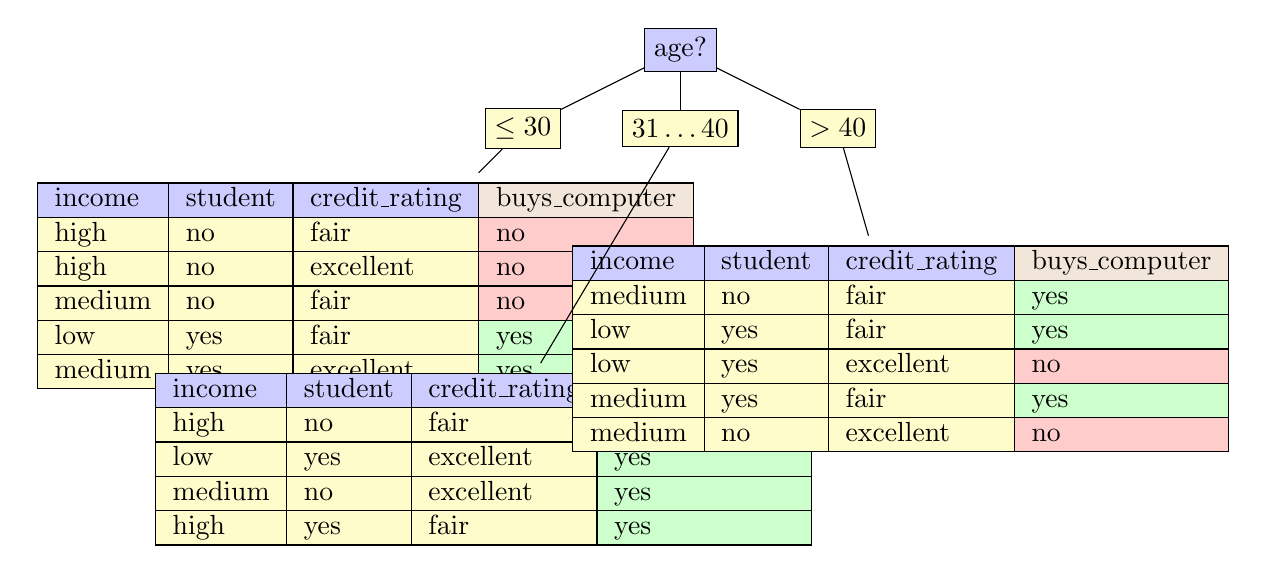
\begin{tikzpicture}
        \node[draw, fill=blue!20] at (0,0) (r) {age?};
        \node[draw, fill=yellow!20] at (-2,-1) (a) {$\leq 30$};
        \node[draw, fill=yellow!20] at (0,-1) (b) {$31\ldots40$};
        \node[draw, fill=yellow!20] at (2,-1) (c) {$>40$};
        \draw (r)--(a);
        \draw (r)--(b);
        \draw (r)--(c);
        \node at (-4,-3) (t1) {
        \begin{tabular}{|l|l|l|l|}
          \hline
          \cellcolor{blue!20}income & \cellcolor{blue!20}student & \cellcolor{blue!20}credit\_rating & \cellcolor{brown!20}buys\_computer \\\hline
          \cellcolor{yellow!20}high & \cellcolor{yellow!20}no & \cellcolor{yellow!20}fair & n\cellcolor{red!20}o \\\hline
          \cellcolor{yellow!20}high & \cellcolor{yellow!20}no & \cellcolor{yellow!20}excellent & \cellcolor{red!20}no \\\hline
          \cellcolor{yellow!20}medium & \cellcolor{yellow!20}no & \cellcolor{yellow!20}fair & \cellcolor{red!20}no \\\hline
          \cellcolor{yellow!20}low & \cellcolor{yellow!20}yes & \cellcolor{yellow!20}fair & \cellcolor{green!20}yes \\\hline
          \cellcolor{yellow!20}medium & \cellcolor{yellow!20}yes & \cellcolor{yellow!20}excellent & \cellcolor{green!20}yes \\\hline
        \end{tabular}
        };
        \node at (-2.5,-5.2) (t3) {
        \begin{tabular}{|l|l|l|l|}
          \hline
          \cellcolor{blue!20}income & \cellcolor{blue!20}student & \cellcolor{blue!20}credit\_rating & \cellcolor{brown!20}buys\_computer \\\hline
          \cellcolor{yellow!20}high & \cellcolor{yellow!20}no & \cellcolor{yellow!20}fair & \cellcolor{green!20}yes \\\hline
          \cellcolor{yellow!20}low & \cellcolor{yellow!20}yes & \cellcolor{yellow!20}excellent & \cellcolor{green!20}yes \\\hline
          \cellcolor{yellow!20}medium & \cellcolor{yellow!20}no & \cellcolor{yellow!20}excellent & \cellcolor{green!20}yes \\\hline
          \cellcolor{yellow!20}high & \cellcolor{yellow!20}yes & \cellcolor{yellow!20}fair & \cellcolor{green!20}yes \\\hline
        \end{tabular}
        };
        \node at (2.8,-3.8) (t2) {
        \begin{tabular}{|l|l|l|l|}
          \hline
          \cellcolor{blue!20}income & \cellcolor{blue!20}student & \cellcolor{blue!20}credit\_rating & \cellcolor{brown!20}buys\_computer \\\hline
          \cellcolor{yellow!20}medium & \cellcolor{yellow!20}no & \cellcolor{yellow!20}fair & \cellcolor{green!20}yes \\\hline
          \cellcolor{yellow!20}low & \cellcolor{yellow!20}yes & \cellcolor{yellow!20}fair & \cellcolor{green!20}yes \\\hline
          \cellcolor{yellow!20}low & \cellcolor{yellow!20}yes & \cellcolor{yellow!20}excellent & \cellcolor{red!20}no \\\hline
          \cellcolor{yellow!20}medium & \cellcolor{yellow!20}yes & \cellcolor{yellow!20}fair & \cellcolor{green!20}yes \\\hline
          \cellcolor{yellow!20}medium & \cellcolor{yellow!20}no & \cellcolor{yellow!20}excellent & \cellcolor{red!20}no \\\hline
        \end{tabular}
        };
        \draw (a)--(t1);
        \draw (c)--(t2);
        \draw (b)--(t3);
      \end{tikzpicture}
    \end{frame}
  }

  {
    \setbeamertemplate{footline}{}
    \begin{frame}{Computing information gain for continuous-valued attributes}
      \begin{itemize}
        \item \textbf{Let attribute A be a continuous-valued attribute.}
        \item \textbf{Must determine the best split point for A.}
        \begin{itemize}
          \item Sort the values of A in increasing order.
          \item Typically, the midpoint between each pair of adjacent values \\ is considered as a possible split point.
          \begin{itemize}
            \item $\frac{a_i+a_{i+1}}{2}$ is the midpoint between the values of $a_i$ and $a_{i+1}$.
          \end{itemize}
          \item The point with the minimum expected information requirement for $A$ \\ is selected as the split point for $A$.
        \end{itemize}
        \item \textbf{Split:}
        \begin{itemize}
          \item $D_1$ is the set of tuples in $D$ satisfying $A \leq$ split point,\\
                and $D_2$ is the set of tuples in $D$ satisfying $A >$ split point.
        \end{itemize}
        \item \textbf{So to say: Discretization as you go along.}
        \begin{itemize}
          \item For this particular purpose.
        \end{itemize}
      \end{itemize}
    \end{frame}
  }

  {
    \setbeamertemplate{footline}{}
    \begin{frame}{Gain ratio for attribute selection (C4.5)}
      \begin{itemize}
        \item \textbf{Information-gain measure is biased towards attributes with a large number of values.}
        \item \textbf{C4.5 (a successor of ID3) uses gain ratio to overcome the problem (normalization to information gain):}
        \begin{align}
          \text{SplitInfo}_A(D) = - \sum_{j=1}^{v} \frac{|D_j|}{|D|} \log_2\left( \frac{|D_j|}{|D|} \right),\\
          \text{GainRatio}(A) = \frac{\text{Gain}(A)}{\text{SplitInfo}_A(D)}.
        \end{align}
        \item Example:
        \begin{align}
          \text{SplitInfo}_{\texttt{income}}(D) &= -\frac{4}{14} \log_2 \left( \frac{4}{14} \right) - \frac{6}{14} \log_2 \left( \frac{6}{14} \right) - \frac{4}{14} \log_2 \left( \frac{4}{14} \right) = 1.557,\\
          \text{GainRatio}(\texttt{income}) &= \frac{0.029}{1.557} = 0.019.
        \end{align}
        \item The attribute with the maximum gain ratio is selected as the splitting attribute.
      \end{itemize}
    \end{frame}
  }

  {
    \setbeamertemplate{footline}{}
    \begin{frame}{Gini index}
      \begin{itemize}
        \item \textbf{Corrado Gini (1884 -- 1965).}
        \begin{itemize}
          \item Italian statistician and sociologist.
        \end{itemize}
        \item \textbf{Also called Gini coefficient.}
        \item \textbf{Measures statistical dispersion.}
        \begin{itemize}
          \item Zero expresses perfect equality where all values are the same.
          \item One expresses maximal inequality among values.
        \end{itemize}
        \item \textbf{Based on the Lorenz curve.}
        \begin{itemize}
          \item Plots the proportion of the total sum of values ($y$-axis) that is cumulatively assigned to the bottom $x\%$ of the population.
          \item Line at $45$ degrees thus represents perfect equality of value distribution.
        \end{itemize}
        \item \textbf{Gini coefficient then is $\ldots$}
        \begin{itemize}
          \item $\ldots$ the ratio of the area that lies between the line of equality and the Lorenz curve over the total area under the line of equality.
        \end{itemize}
      \end{itemize}
    \end{frame}
  }

  {
    \setbeamertemplate{footline}{}
    \begin{frame}{Gini index (II)}
      \centering
      Example: Distribution of incomes.\\[0.5cm]
      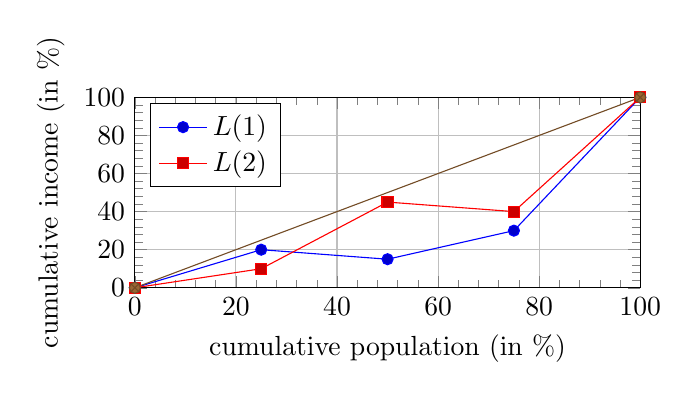
\begin{tikzpicture}
      \begin{axis}[
          xmin=0, xmax=100,
          ymin=0, ymax=100,
          minor tick num = 4,
          grid,
          ylabel = cumulative income (in \%),
          xlabel = cumulative population (in \%),
          legend style={legend pos=north west},
          ]
      \addplot plot
          coordinates {(0,0) (25,20) (50,15) (75,30) (100,100)};
      \addplot plot
          coordinates {(0,0) (25,10) (50,45) (75,40) (100,100)};
      \addplot plot [thin]
          coordinates {(0,0) (100,100)};
      \legend{$L(1)$,$L(2)$}
      \end{axis}
    \end{tikzpicture}
    \end{frame}
  }

  {
    \setbeamertemplate{footline}{}
    \begin{frame}{Gini index (CART, IBM IntelligentMiner)}
      \begin{itemize}
        \item \textbf{If a dataset D contains examples from n classes, Gini index gini(D) is defined as:}
        \begin{align}
          \text{gini}(D) = 1-\sum_{j=1}^{n} p_j^2,
        \end{align}
        where $p_j$ is the relative frequency of class $j$ in $D$.
        \item \textbf{If a dataset $D$ is split on $A$ into two subsets $D_1$ and $D_2$, the Gini index $\text{gini}(D)$ is defined as}
        \begin{align}
          \text{gini}_A(D) = \frac{|D_1|}{|D|}\text{gini}(D_1)+\frac{|D_2|}{|D|}\text{gini}(D_2).
        \end{align}
        \item \textbf{Reduction in impurity:}
        \begin{align}
          \Delta \text{gini}_A(A) = \text{gini}(D)-\text{gini}_A(D).
        \end{align}
        \item \textbf{The attribute $A$ provides the smallest $\text{gini}_A(D)$ (or the largest reduction in impurity) \\ is chosen to split the node.}
        \begin{itemize}
          \item Need to enumerate all the possible splitting points for each attribute.
        \end{itemize}
      \end{itemize}
    \end{frame}
  }


  {
    \setbeamertemplate{footline}{}
    \begin{frame}{Computation of Gini index}
      \begin{itemize}
        \item \textbf{Example:}
        \begin{itemize}
          \item $D$ has $9$ tuples in $\text{buys\_computer} =$ "yes" and 5 in "no", thus
          \begin{align}
            \text{gini}(D) = 1 - \left( \frac{9}{14} \right)^2 - \left( \frac{5}{14} \right) = 0.459.
          \end{align}
        \end{itemize}
        \item Suppose the attribute $\texttt{income}$ partitions $D$ \\ into $10$ in $D_1:\{\texttt{low,medium}\}$ and $4$ in $D_2: \{\texttt{high}\}$:
        \begin{align}
          &\text{gini}(D\vert_{D[\texttt{income}]="medium", "low"}) \\
          &= \left( \frac{10}{14} \right) \text{gini}(D_1) + \frac{4}{14} \text{gini}(D_2)\\
          &=\frac{10}{14} \left(1-\left( \frac{7}{10} \right)^2 - \left( \frac{3}{10} \right)^2 \right) + \frac{4}{14} \left( 1-\left( \frac{2}{4} \right)^2 - \left( \frac{2}{4} \right)^2 \right) =\\
          &= 0.443 = \text{gini}(D\vert_{D[\texttt{income}]="high"}).
        \end{align}
      \end{itemize}
    \end{frame}
  }

  {
    \setbeamertemplate{footline}{}
    \begin{frame}{Computation of Gini index (II)}
      \begin{itemize}
        \item \textbf{Example (cont.):}
        \begin{itemize}
          \item $\text{gini}(D\vert_{D[\texttt{income}]="low", "high"}) = 0.458$,\\
                $\text{gini}(D\vert_{D[\texttt{income}]="medium", "high"}) = 0.450.$
          \item Thus, split on the \{"low","medium"\} and \{"high"\}, since it has the lowest gini index.
        \end{itemize}
        \item \textbf{All attributes are assumed continuous-valued.}
        \item \textbf{May need other tools, e.g. clustering, to get the possible split values.}
        \item \textbf{Can be modified for categorical attributes.}
      \end{itemize}
    \end{frame}
  }

  {
    \setbeamertemplate{footline}{}
    \begin{frame}{Computation of Gini index (II)}
      \begin{itemize}
        \item \textbf{The three measures, in general, return good results, but}
        \begin{itemize}
          \item \textbf{\color{airforceblue}Information gain:}
          \begin{itemize}
            \item Biased towards multi-valued attributes.
          \end{itemize}
          \item \textbf{\color{airforceblue}Gain ratio:}
          \begin{itemize}
            \item Tends to prefer unbalanced splits in which one partition is much smaller than the others.
          \end{itemize}
          \item \textbf{\color{airforceblue}Gini index:}
          \begin{itemize}
            \item Biased to multi-valued attributes.
            \item Has difficulty when number of classes is large.
            \item Tends to favor tests that result in equal-sized partitions and purity in both partitions.
          \end{itemize}
        \end{itemize}
      \end{itemize}
    \end{frame}
  }

  {
    \setbeamertemplate{footline}{}
    \begin{frame}{Other attribute-selection measures}
      \begin{itemize}
        \item \textbf{CHAID:}
        \begin{itemize}
          \item A popular decision-tree algorithm, measure based on $\chi^2$ test for independence.
        \end{itemize}
        \item \textbf{C-SEP:}
        \begin{itemize}
          \item Performs better than information gain and Gini index in certain cases.
        \end{itemize}
        \item \textbf{G-statistic:}
        \begin{itemize}
          \item Has a close approximation to $\chi^2$ distribution.
        \end{itemize}
        \item \textbf{MDL (Minimal Description Length) principle:}
        \begin{itemize}
          \item I.e. the simplest solution is preferred.
          \item The best tree is the one that requires the fewest number of bits to both (1) encode the tree and (2) encode the exceptions to the tree.
        \end{itemize}
        \item \textbf{Multivariate splits:}
        \begin{itemize}
          \item Partitioning based on multiple variable combinations.
          \item CART: finds multivariate splits based on a linear combination of attributes.
        \end{itemize}
        \item \textbf{Which attribute-selection measure is the best?}
        \begin{itemize}
          \item Most give good results, none is significantly superior to others.
        \end{itemize}
      \end{itemize}
    \end{frame}
  }

  {
    \setbeamertemplate{footline}{}
    \begin{frame}{Overfitting and tree pruning}
      \begin{itemize}
        \item \textbf{Overfitting: An induced tree may overfit the training data.}
        \begin{itemize}
          \item Too many branches, some may reflect anomalies due to noise or outliers.
          \item Poor accuracy for unseen samples.
        \end{itemize}
        \item \textbf{Two approaches to avoid overfitting:}
        \begin{itemize}
          \item \textbf{\color{airforceblue}Prepruning:}
          \begin{itemize}
            \item Halt tree construction early.\\
                  Do not split a node, if this would result in the goodness measure falling below a threshold.
            \item Difficult to choose an appropriate threshold.
          \end{itemize}
          \item \textbf{\color{airforceblue}Postpruning:}
          \begin{itemize}
            \item Remove branches from a "fully grown" tree.\\
                  Get a sequence of progressively pruned trees.
            \item Use a set of data different from the training data to decide which is the "best pruned tree."
          \end{itemize}
        \end{itemize}
      \end{itemize}
    \end{frame}
  }

  {
    \setbeamertemplate{footline}{}
    \begin{frame}{Enhancements to Basic Decision-Tree Induction}
      \begin{itemize}
        \item \textbf{Allow for} \textbf{\color{airforceblue}continuous-valued attributes.}
        \begin{itemize}
          \item Dynamically define new discrete-valued attributes that partition the values of continuous-valued attributes into a discrete set of intervals.
        \end{itemize}
        \item \textbf{Handle} \textbf{\color{airforceblue}missing attribute values.}
        \begin{itemize}
          \item Assign the most common value of the attribute.
          \item Assign probability to each of the possible values.
        \end{itemize}
      \item \textbf{\color{airforceblue}Attribute construction.}
      \begin{itemize}
        \item Create new attributes based on existing ones that are sparsely represented.
        \item This reduces fragmentation, repetition, and replication.
      \end{itemize}
      \end{itemize}
    \end{frame}
  }

  {
    \setbeamertemplate{footline}{}
    \begin{frame}{Classification in large databases}
      \begin{itemize}
        \item \textbf{Classification -- a classical problem extensively \\ studied by statisticians and machine-learning researchers.}
        \item \textbf{Scalability:}
        \begin{itemize}
          \item Classifying datasets with millions of examples and \\ hundreds of attributes with reasonable speed.
        \end{itemize}
        \item \textbf{Why is decision-tree induction popular?}
        \begin{itemize}
          \item Relatively fast learning speed (compared to other classification methods).
          \item Convertible to simple and easy-to-understand classification rules.
          \item Can use SQL queries for accessing databases.
          \item Classification accuracy comparable with other methods.
        \end{itemize}
        \item \textbf{RainForest (Gehrke, Ramakrishnan \& Ganti, VLDB'98).}
        \begin{itemize}
          \item Builds an AVC-list (attribute, value, class label).
        \end{itemize}
      \end{itemize}
    \end{frame}
  }

  {
    \setbeamertemplate{footline}{}
    \begin{frame}{Scalability framework for RainForest}
      \begin{itemize}
        \item \textbf{Separates the scalability aspects from the criteria that determine the quality of the tree.}
        \item \textbf{Builds an} \textbf{\color{airforceblue}AVC-list:}.
        \begin{itemize}
          \item AVC (Attribute, Value, Class\_label).
        \end{itemize}
        \item \textbf{\color{airforceblue}AVC-set} \textbf{(of an attribute X):}
        \begin{itemize}
          \item Projection of training dataset onto the attribute $X$ and class label where counts of individual class label are aggregated.
        \end{itemize}
        \item \textbf{\color{airforceblue}AVC-group} \textbf{(of a node n):}
        \begin{itemize}
          \item Set of AVC-sets of all predictor attributes at the node $n$.
        \end{itemize}
      \end{itemize}
    \end{frame}
  }

  {
    \setbeamertemplate{footline}{}
    \begin{frame}{RainForest: training set and its AVC-sets}
      \begin{columns}
        \begin{column}{0.6\textwidth}
          \begin{tabular}{|c|l|c|l|c|}
            \hline
            \cellcolor{blue!20}age & \cellcolor{blue!20}income & \cellcolor{blue!20}student & \cellcolor{blue!20}credit\_rating & \cellcolor{brown!20}buys\_computer \\\hline
            \cellcolor{yellow!20}$\leq30$ & \cellcolor{yellow!20}high & \cellcolor{yellow!20}no & \cellcolor{yellow!20}fair & \cellcolor{red!20}no \\\hline
            \cellcolor{yellow!20}$\leq30$ & \cellcolor{yellow!20}high & \cellcolor{yellow!20}no & \cellcolor{yellow!20}excellent & \cellcolor{red!20}no \\\hline
            \cellcolor{yellow!20}$31\ldots40$ & \cellcolor{yellow!20}high & \cellcolor{yellow!20}no & \cellcolor{yellow!20}fair & \cellcolor{green!20}yes \\\hline
            \cellcolor{yellow!20}$>40$ & \cellcolor{yellow!20}medium & \cellcolor{yellow!20}no & \cellcolor{yellow!20}fair & \cellcolor{green!20}yes \\\hline
            \cellcolor{yellow!20}$>40$ & \cellcolor{yellow!20}low & \cellcolor{yellow!20}yes & \cellcolor{yellow!20}fair & \cellcolor{green!20}yes \\\hline
            \cellcolor{yellow!20}$>40$ & \cellcolor{yellow!20}low & \cellcolor{yellow!20}yes & \cellcolor{yellow!20}excellent & \cellcolor{red!20}no \\\hline
            \cellcolor{yellow!20}$31\ldots40$ & \cellcolor{yellow!20}low & \cellcolor{yellow!20}yes & \cellcolor{yellow!20}excellent & \cellcolor{green!20}yes \\\hline
            \cellcolor{yellow!20}$\leq30$ & \cellcolor{yellow!20}medium & \cellcolor{yellow!20}no & \cellcolor{yellow!20}fair & \cellcolor{red!20}no \\\hline
            \cellcolor{yellow!20}$\leq30$ & \cellcolor{yellow!20}low & \cellcolor{yellow!20}yes & \cellcolor{yellow!20}fair & \cellcolor{green!20}yes \\\hline
            \cellcolor{yellow!20}$>40$ & \cellcolor{yellow!20}medium & \cellcolor{yellow!20}yes & \cellcolor{yellow!20}fair & \cellcolor{green!20}yes \\\hline
            \cellcolor{yellow!20}$\leq30$ & \cellcolor{yellow!20}medium & \cellcolor{yellow!20}yes & \cellcolor{yellow!20}excellent & \cellcolor{green!20}yes \\\hline
            \cellcolor{yellow!20}$31\ldots40$ & \cellcolor{yellow!20}medium & \cellcolor{yellow!20}no & \cellcolor{yellow!20}excellent & \cellcolor{green!20}yes \\\hline
            \cellcolor{yellow!20}$31\ldots40$ & \cellcolor{yellow!20}high & \cellcolor{yellow!20}yes & \cellcolor{yellow!20}fair & \cellcolor{green!20}yes \\\hline
            \cellcolor{yellow!20}$>40$ & \cellcolor{yellow!20}medium & \cellcolor{yellow!20}no & \cellcolor{yellow!20}excellent & \cellcolor{red!20}no \\\hline
          \end{tabular}
        \end{column}
        \begin{column}{0.3\textwidth}
          \vspace{-3cm}

          \centering
          AVC-set on age:\\
          \begin{tabular}{|c|c|c|}
            \hline
            age & yes & no \\\hline
            $\leq 30$ & 2 & 3 \\\hline
            $31\ldots40$ & 4 & 0 \\\hline
            $>40$ & 3 & 2 \\\hline
          \end{tabular}\\[1cm]
          AVC-set on income:\\
          \begin{tabular}{|c|c|c|}
            \hline
            income & yes & no \\\hline
            high & 2 & 2 \\\hline
            medium & 4 & 2 \\\hline
            low & 3 & 1 \\\hline
          \end{tabular}
        \end{column}
      \end{columns}
    \end{frame}
  }

  {
    \setbeamertemplate{footline}{}
    \begin{frame}{RainForest: training set and its AVC-sets (II)}
      \begin{columns}
        \begin{column}{0.6\textwidth}
          \begin{tabular}{|c|l|c|l|c|}
            \hline
            \cellcolor{blue!20}age & \cellcolor{blue!20}income & \cellcolor{blue!20}student & \cellcolor{blue!20}credit\_rating & \cellcolor{brown!20}buys\_computer \\\hline
            \cellcolor{yellow!20}$\leq30$ & \cellcolor{yellow!20}high & \cellcolor{yellow!20}no & \cellcolor{yellow!20}fair & \cellcolor{red!20}no \\\hline
            \cellcolor{yellow!20}$\leq30$ & \cellcolor{yellow!20}high & \cellcolor{yellow!20}no & \cellcolor{yellow!20}excellent & \cellcolor{red!20}no \\\hline
            \cellcolor{yellow!20}$31\ldots40$ & \cellcolor{yellow!20}high & \cellcolor{yellow!20}no & \cellcolor{yellow!20}fair & \cellcolor{green!20}yes \\\hline
            \cellcolor{yellow!20}$>40$ & \cellcolor{yellow!20}medium & \cellcolor{yellow!20}no & \cellcolor{yellow!20}fair & \cellcolor{green!20}yes \\\hline
            \cellcolor{yellow!20}$>40$ & \cellcolor{yellow!20}low & \cellcolor{yellow!20}yes & \cellcolor{yellow!20}fair & \cellcolor{green!20}yes \\\hline
            \cellcolor{yellow!20}$>40$ & \cellcolor{yellow!20}low & \cellcolor{yellow!20}yes & \cellcolor{yellow!20}excellent & \cellcolor{red!20}no \\\hline
            \cellcolor{yellow!20}$31\ldots40$ & \cellcolor{yellow!20}low & \cellcolor{yellow!20}yes & \cellcolor{yellow!20}excellent & \cellcolor{green!20}yes \\\hline
            \cellcolor{yellow!20}$\leq30$ & \cellcolor{yellow!20}medium & \cellcolor{yellow!20}no & \cellcolor{yellow!20}fair & \cellcolor{red!20}no \\\hline
            \cellcolor{yellow!20}$\leq30$ & \cellcolor{yellow!20}low & \cellcolor{yellow!20}yes & \cellcolor{yellow!20}fair & \cellcolor{green!20}yes \\\hline
            \cellcolor{yellow!20}$>40$ & \cellcolor{yellow!20}medium & \cellcolor{yellow!20}yes & \cellcolor{yellow!20}fair & \cellcolor{green!20}yes \\\hline
            \cellcolor{yellow!20}$\leq30$ & \cellcolor{yellow!20}medium & \cellcolor{yellow!20}yes & \cellcolor{yellow!20}excellent & \cellcolor{green!20}yes \\\hline
            \cellcolor{yellow!20}$31\ldots40$ & \cellcolor{yellow!20}medium & \cellcolor{yellow!20}no & \cellcolor{yellow!20}excellent & \cellcolor{green!20}yes \\\hline
            \cellcolor{yellow!20}$31\ldots40$ & \cellcolor{yellow!20}high & \cellcolor{yellow!20}yes & \cellcolor{yellow!20}fair & \cellcolor{green!20}yes \\\hline
            \cellcolor{yellow!20}$>40$ & \cellcolor{yellow!20}medium & \cellcolor{yellow!20}no & \cellcolor{yellow!20}excellent & \cellcolor{red!20}no \\\hline
          \end{tabular}
        \end{column}
        \begin{column}{0.3\textwidth}
          \vspace{-3cm}

          \centering
          AVC-set on student:\\
          \begin{tabular}{|c|c|c|}
            \hline
            student & yes & no \\\hline
            yes & 6 & 1 \\\hline
            no & 3 & 4 \\\hline
          \end{tabular}\\[1cm]
          AVC-set on credit\_rating:\\
          \begin{tabular}{|c|c|c|}
            \hline
            credit\_rating & yes & no \\\hline
            fair & 6 & 2 \\\hline
            excellent & 3 & 3 \\\hline
          \end{tabular}
        \end{column}
      \end{columns}
    \end{frame}
  }


  { % Questions?
    \setbeamertemplate{footline}{}
    \begin{frame}[c]
      \begin{center}
        Thank you for your attention.\\
        {\bf Any questions about the sixt chapter?}\\[0.5cm]
        Ask them now, or again, drop me a line: \\
        \faSendO \ \texttt{luciano.melodia@fau.de}.
      \end{center}
    \end{frame}
  }
\end{document}
